\chapter{Background}\label{sec:background}

This section gives brief background of the methods used for my these.
Section~\ref{sec:back:hubo-ach} describes why inter-process communication (IPC) is used for the Hubo-Ach control system and a brief background of different IPC methods.
Section~\ref{sec:hubo-ach} give this background in greater detail.
Section~\ref{sec:back:ik} and \ref{sec:back:eefvelos} gives the background for the methods used for inverse kinematics and throwing on high DOF robots.
This is the background to the development of the control system that made Hubo throw the first pitch at a Major League Baseball game in 2012 as seen in Section~\ref{sec:hubo-ach} and multiple examples given in Section~\ref{sec:simpleExamples}.
Finally Section~\ref{sec:zmp} gives a brief description of the Zero Moment Point criteria which is used for humanoid walking and shown in the examples in Section~\ref{sec:simpleExamples}.

		
		\section{Hubo-Ach: Multi-Process and Interprocess Comunication}\label{sec:back:hubo-ach}
`	    		
This section gives a quick background to why inter-process communication (IPC) is used for the Hubo-Ach control system and a brief background of different IPC methods.
Section~\ref{sec:hubo-ach} give this background in greater detail.

The idea for a Control Architecture for High DOF robots stems from a gap in physical implementation of control algorithms for robot hardware.
The simplest approach to developing robot software is to integrate all functionality in one program.  
This functionality includes the following controllers:
\begin{multicols}{2}
\begin{itemize}
\item Hardware Control
\item Perception
\item Planning
\item Kinematics
\item etc.
\end{itemize}
\end{multicols}

If all of this functionality is in one process then it has the benefit of freedom of inter process communication latency.
However being in one process also means that if one of the controllers lags or faults it cause the entire controller to lag or fault.
This is of great concern if a non-priority controller such as vision processing faults causing a priority controller such as a balance controller, to fail.
This will cause the robot to fall.
How is this fixed?
One solution and my proposed solution is to use multiple processes and IPC methods.
Inter-process communication is a method of exchanging data between multiple processes.
Typical POSIX methods give you the \textbf{oldest} information first and have locks on the memory when processes are writing to it.
An overview of these mechanisms are given in \cite{stevens2005advanced}.

Robots work in the physical world. 
More recent information is more important to it then older.
In most cases it is acceptable to know the most recent data and never read any of the older data.
This would happen if your sensors update at a faster rate then that of the robot.
Typically robot actuators have a bandwidth much much lower then that of a modern computer.
If sensor information is shared using traditional shared memory over POSIX methods the controller would have to read the older information before it reaches the information it is most interested in, the newest data.
This is known effect but new concern for robot controllers called head of line blocking\cite{ach}.

It is desired to make a multi-process controller that can share data between multiple processes with low-latency and no head of line blocking.
There are a few IPCs that offer no head of line blocking and low-latency.  
A description of each IPC type is in Section~\ref{sec:hubo-ach}.
Table~\ref{table:ipc} shows a full comparison of the different IPC types.
%After much research (inserte examples here) it was found that the Ach IPC wuld best fit my needs.

My thesis Hubo-Ach is a multi-process control system that uses IPC methods to communicate between processes.
Section~\ref{sec:hubo-ach} describes Hubo-Ach in detail.



		\section{Kinematic Planning}\label{sec:back:ik}
			Kinematic planning focuses on creating and testing valid trajectories for series kinematic manipulators.
The focus of this research is on high degree of freedom (DOF), high-gain, position controlled mechanisms.
The works are chosen as it pertains to end-effector velocity control.
Throwing and hitting are examples of end-effector velocity control.  
The goal is to have the end-effector moving at a specific rate in a specific direction.
In most cases it demands whole-body coordination to achieve a desired end-effector velocity.  
Whole-body coordination is different for planted robots and un-planted robots.  


\noindent \textit{Planted robots} are robots where the base is attached to the ground or the base is significantly more massive then the manipulator.
Planted robots do not have to worry about balance consternates. 

\noindent \textit{Un-planted robots} are robots that have an manipulator that is not significantly ligher then the base.  
In addition the robot is not physically attached to the ground.
This results in the robot needing to satisfy balance constraints.
In the static case if the robot satisfies the zero moment point (ZMP) criteria it will remain stable~\cite{5686276}.
When the manipulator moves quickly, as in the case of pitching or throwing, such upper-body motions if not coordinated with the lower-body, can cause the humanoid to lose balance.  



%The goal of this work is to show the creation of collision free trajectories for end-effector velocity control, the first step in our overarching goal of creating a system with the ability to throw objects and retain balance.  Towards this, Section~\ref{sec:selfCollision} will discuss our method of detecting self collisions.  Section~\ref{sec:rarea} describes the creation of the robot's sparse reachable map (SRM), a map in $R^3$ of the reachable points. through setting random values to the robot in joint space that takes into account joint limitations and self collisions.  Section~\ref{sec:trajGen} shows the creation of a throwing trajectory in $R^3$ and placing it withing the robot's reachable area using the SRM.  Section~\ref{sec:ik} explains the inverse kinematics used to convert the throwing trajectory in $R^3$ to joint space for this high degree of freedom humanoid robot.  Section~\ref{sec:trap} describes the creation of the approach from the initial pose to the starting pose of the throwing trajectory using a variant of trapezoidal motion control to keep within the actuators' physical limitations.  Section~\ref{sec:exp} features experiments to demonstrate the successful execution of this paper's goal.  Section~\ref{sec:conc} concludes the paper and comments on future work.
		\section{End-Effector Velocity Control}\label{sec:back:eefvelos}
			End-effector velocity control (EEVC) is the act of moving your manipulator at a given speed through space at a given velocity.
EEVC is being looked at as the mass of the end-effector does not change.
Thus by controlling the velocity we also control the inertia.
In addition I will be exploring EEVC as it pertains to manipulating objects.
Through my research I have found that end-effector velocity control can be broken up into four major categories:
\textit{Time and location sensitive}, \textit{location sensitive}, \textit{time sensitive}, and \textit{time and location insensitive}.\\


\noindent \textbf{Time and Location Sensitive}: 
If your velocity control is time and location sensitive it means that your end effector needs to have a given velocity at a specific time in a specific location or the task fales.
Hitting a baseball with a bat is an example of \textit{time and location sensitive}  EEVC.
If the bat has the correct velocity but not at the correct time it will not hit the ball or the ball will not go in the desired place.  
The same goes for if it does not have the correct location but does have the correct velocity.
It is important to note that the manipulator only has instantaneous control over the object at the instant of contact.
Other examples include playing the piano, hitting a tennis ball with a racquet, a moving soccer ball with a foot or any other task that requires to \textit{hit} a \textit{moving} object.\\


\noindent \textbf{Location Sensitive}:
If your velocity control is location sensitive it means that it only matters that the velocity occurs at a given location.
The time it takes to reach that velocity will not effect the results.
Hitting a nail with a hammer is a prime example of location sensitive EEVC.  
The nail is not moving but it does need to be hit in a given location with a given velocity.
The vector of the velocity is determined by the required angle the nail needs to be hit at.
In this example the nail is not time dependent and can be hit any time.
Hitting it a $t=N$ or $t=N+1$ will not effect the results.
It is important to note that the manipulator only has instantaneous control over the object at the instant of contact.
Other examples of location sensitive end-effector velocity control are hitting a golf ball with a club, hitting a pool ball with the cue, and other activities that require a given location and direction of manipulation but are not time dependent.\\


\noindent \textbf{Time Sensitive}: 
If the location were the end-effector achieves a given velocity is not required to complete the task but the time when it happens is required it is considered \textit{time sensitive} EEVC. 
This means that the end-effector can move in any region it desired as long as the end effector achieves a given velocity at a given time.
The end-effecter's velocity can be dependent on the location achieved but the location is an independent variable and the velocity is the dependent variable.
It is important to note that the manipulator control over the object during the entirety of the motion.
This typically means that the manipulator is holding the object until the release stage.
An example of this is throwing a baseball to first base to get someone out.
Throwing the ball side arm, over arm, or even underarm does not matter as long at it is released at the correct time with the correct velocity to get it ball to the first-baseman to get the runner out.
Other example of time sensitive EEVC are any other instance where an object is thrown within a given time. \\




\noindent \textbf{Time and Location Insensitive}:
If the location and the time of when the end-effector achieves a given velocity does not matter it is considered time and location insensitive.  
The end-effecter's velocity can be dependent on the location achieved but the location is an independent variable and the velocity is the dependent variable.
In this case the manipulator has control over the object until the release stage.
Examples of this would be pitching a baseball, bowling, throwing a grenade or horseshoes etc.
Throwing is an example of when the end-effector's velocity holds a higher priority over the position.  


Mechanisms with only a single degree of freedom are restricted to throwing in a plane.   2-DOF mechanisms are able to throw in $R^3$ space with the correct kinematic structure.
Such a mechanism can choose its release point or its end-effector velocity but not both.
Mechanisms containing 3 or more DOF with the correct kinematic structure are able to throw in $R^3$ and choose both the release point and the end-effector velocity simultaneously. 

In recent work Mori et al. \cite{5152525} has show his ability to control the translational velocity, angular velocity and direction in a 2-dimension plane independently with a single DOF mechanism.
The only input is torque to the manipulator.
The concept consists is to map the input torque that will change only one of the kinimatic variables and not the other two.
This map is done over a given space and thus you can independently chose your translational and angular velocity as well as direction as long as it is in the valid search space.
The manipulator and a search space example can be seen in Fig.~\ref{fig:mori}. 

\begin{figure}[thpb]
  \centering
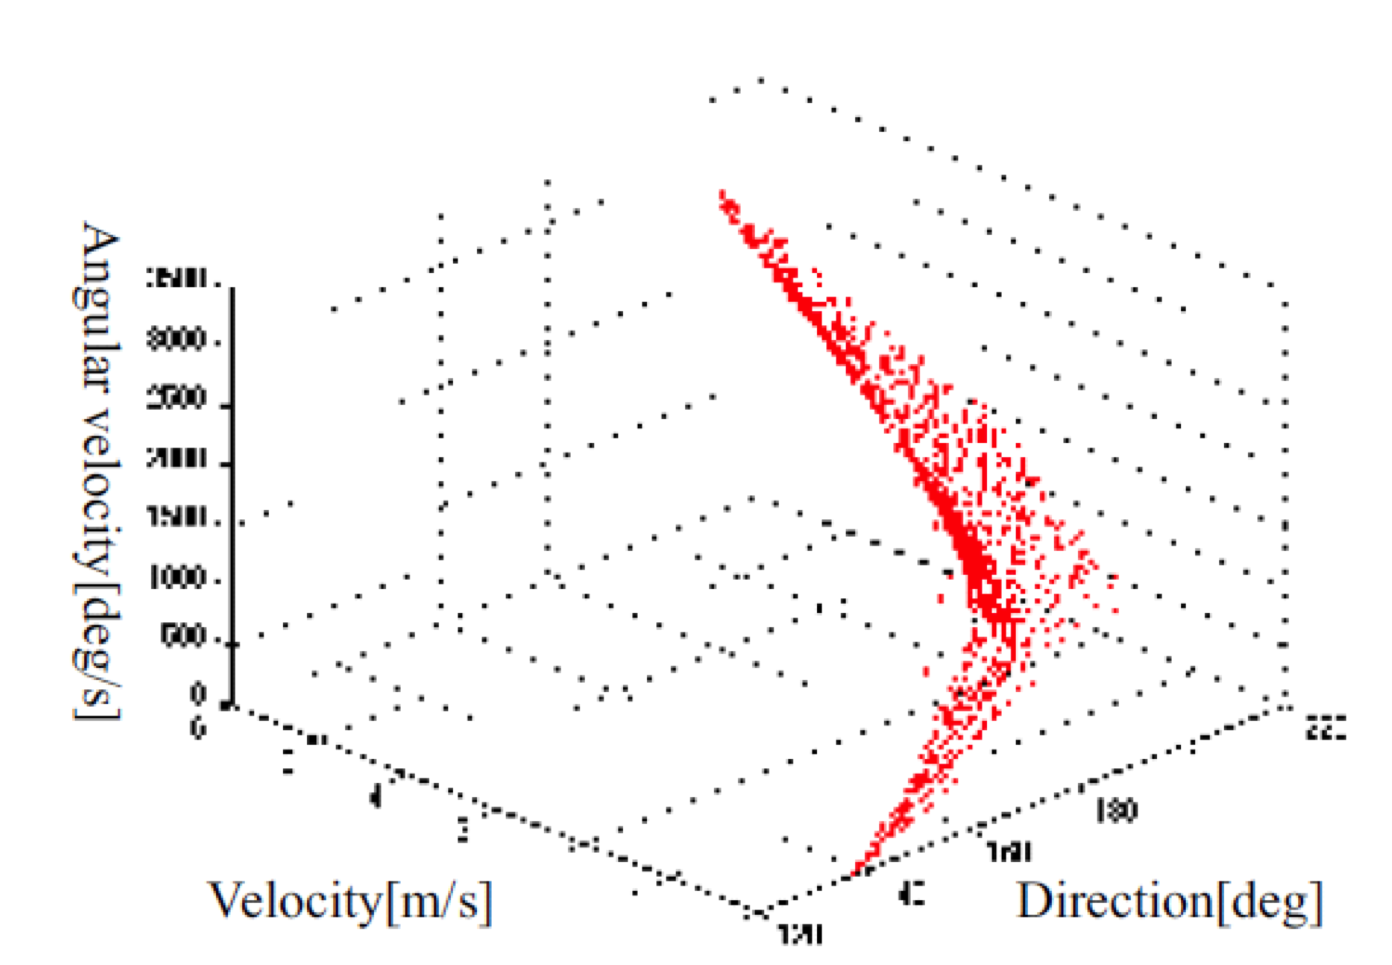
\includegraphics[width=0.4\columnwidth]{./background/pix/mori2.png}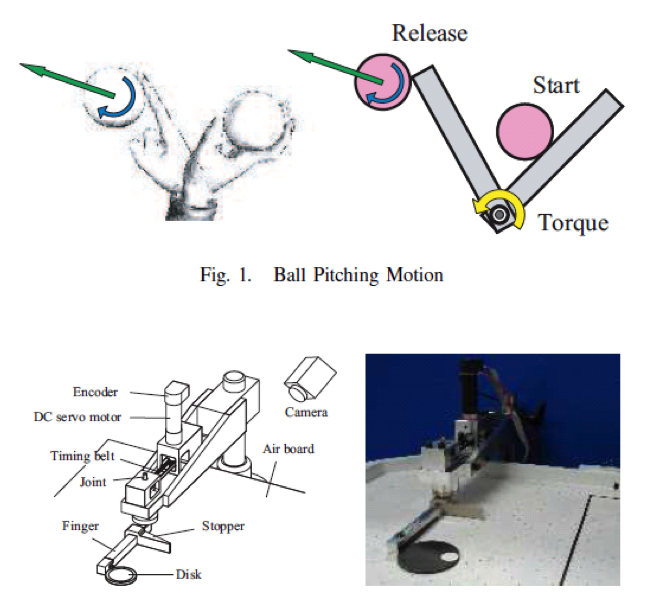
\includegraphics[width=0.4\columnwidth]{./background/pix/mori1.png}
  \caption{Map of the input torque that will change only one of the kinimatic variables and not the other two.
This map is done over a given space and thus you can independently chose your translational and angular velocity as well as direction as long as it is in the valid search space.}
  \label{fig:mori}
\end{figure}


Senoo et al.\cite{4651142} used a torque controlled 3-DOF arm to create a high speed throwing trajectory.
This arm falls into the \textit{time and location insensitive} category of throwing.
Senoo used a kinematic chain approach based on how humans throw.  
Doing this Senoo was able to achieved an end-effector velocity of 6.0 $m/s$ and can throw in $R^3$ space.
This is done via the use of a planted robot arm made by Barret Technology Inc consisting of 3-DOF with a $360^o$ rotation base yaw actuator, see Fig.~\ref{fig:senoo}. 
 

\begin{figure}[thpb]
  \centering
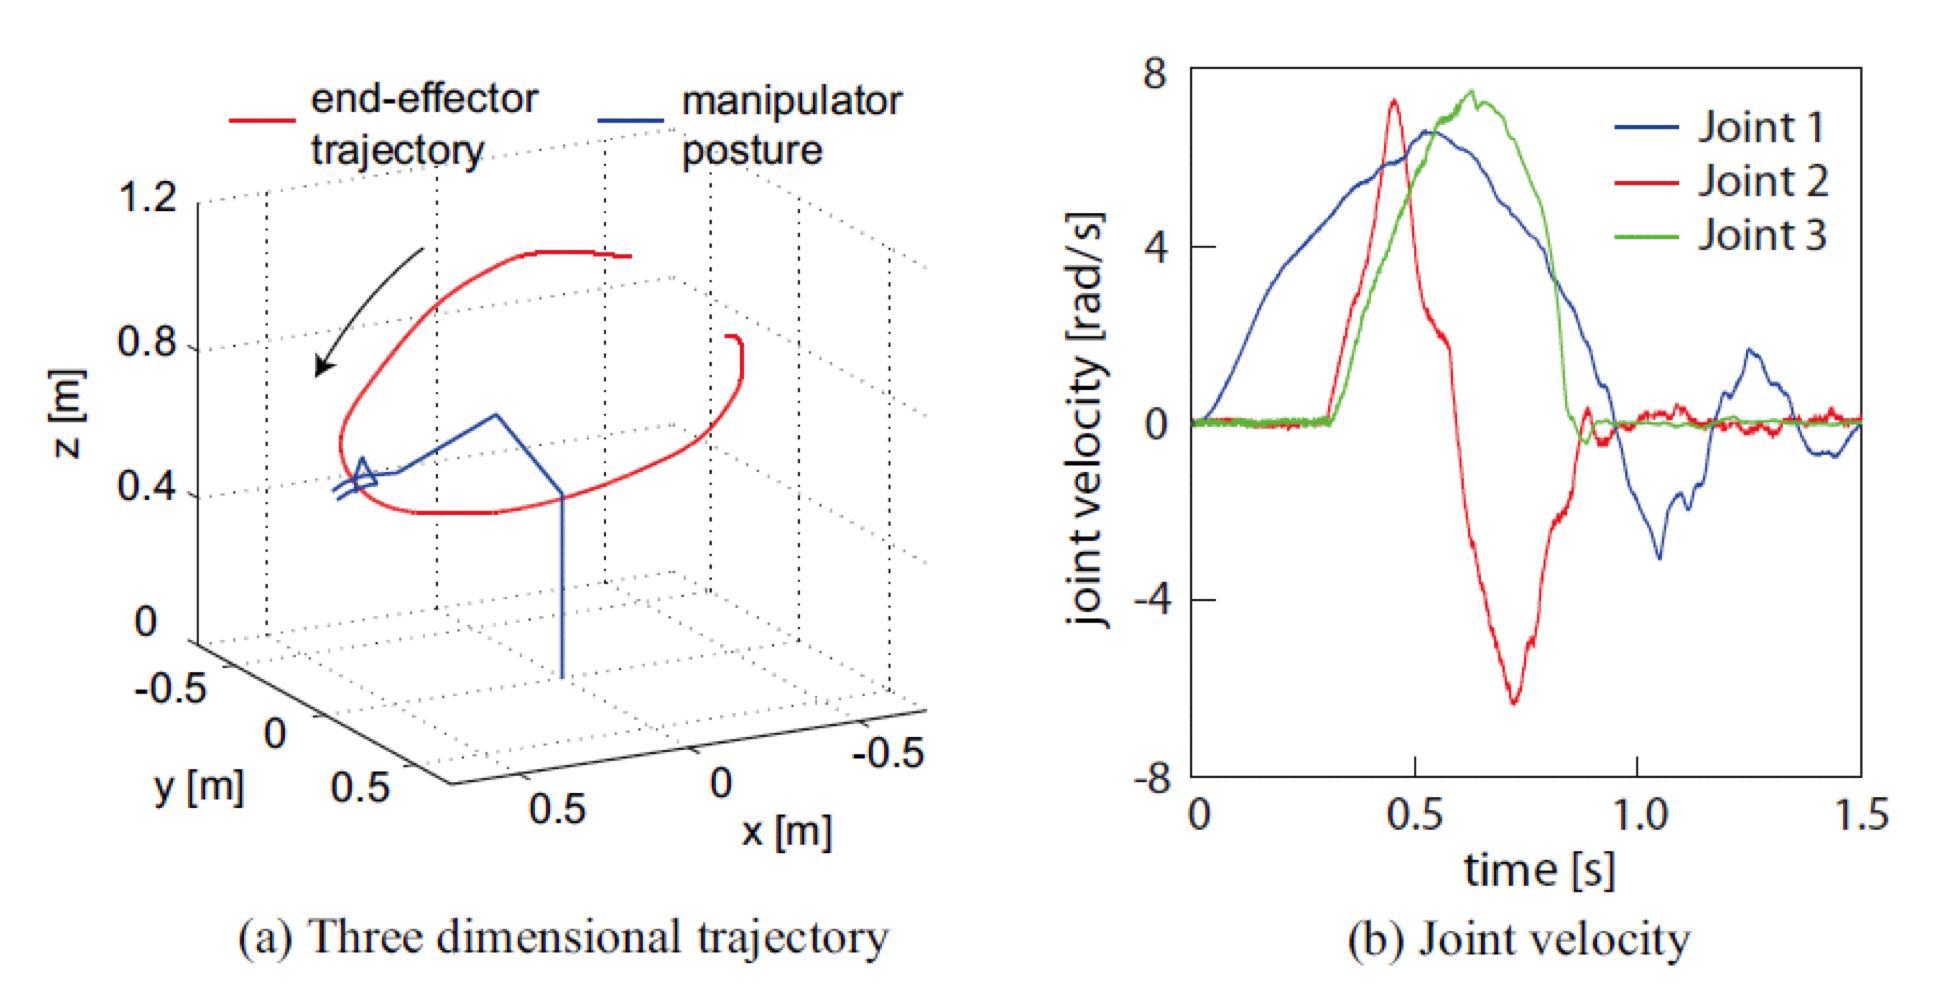
\includegraphics[width=0.6\columnwidth]{./background/pix/senoo2.png}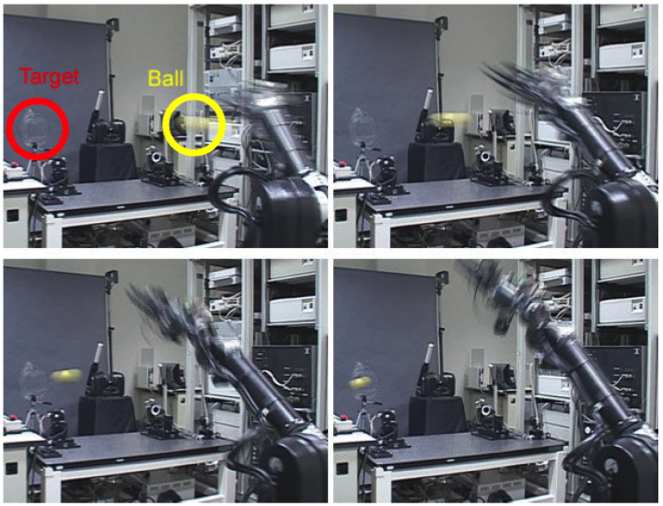
\includegraphics[width=0.4\columnwidth]{./background/pix/senoo1.png}
  \caption{3-DOF arm achieving an end-effector velocity of 6.0 $m/s$ and can throw in $R^3$ space.
This is done via the use of a planted robot arm made by Barret Technology Inc with a $360^o$ rotation base yaw actuator}
  \label{fig:senoo}
\end{figure}
 

Low degree of freedom throwing machines/robots are common.  
Typical throwing robots have between one and three degrees of freedom (DOF)~\cite{509405, Lynch97dynamicnonprehensile, 5152525, 509335, springerlink:10.1007/s10015-006-0401-0}.
All of these mechanisms are limited to throwing in a plane.   



These low degree of freedom throwing robots are either physically attached/planted to the mechanical ground or have a base that is significantly more massive then the arm.  

Haddadin et al.\cite{6094757} used their 7-DOF arm and a 6-DOF force torque sensor with standard feedback methods to dribble a basket ball.  
In addition Zhikun et al.~\cite{6094892} used reinforcement learning to teach their 7-DOF planted robot arm to play ping-pong.  
Likewise Schaal et al.~\cite{schaal01/BIRG} taught their high degree of freedom (30-DOF) humanoid to hit a tennis ball using an on-line special statistical learning methods.
Visual feedback was used in the basketball throwing robot by Hu et al.~\cite{5649335} achieving accuracy of 99\%.  
All of the latter robots were fixed to the ground to guarantee stability.

Kim et al. \cite{5686315,JooH2011438} takes the research to the next level with finding optimal overhand and sidearm throwing motions for a high degree of freedom humanoid computer model.  The model consists of 55-DOF and is not fixed to mechanical ground or a massive base.  Motor torques are then calculated to create both sidearm and overhand throws that continuously satisfies the zero-moment-point stability criteria~\cite{4309277}.  



%			\input{background/FaultDetection.tex}
		\section{Balancing: Zero-Moment-Point (ZMP)}\label{sec:zmp}
			\chapter{Balancing: Zero-Moment-Point (ZMP)}\label{sec:zmp}
The past years of research in humanoids robotics has resulted in a stability criteria that must be followed for bipedal robots to stay stable.
This is known as the Zero Moment Point criteria commonly referred to as ZMP \cite{zmp35}.
ZMP is ubiquitous in the humanoid robotics community.
The ZMP criteria states that a system is statically stable (balanced) if there is no moment acting on the connection between the end effectors touching the ground and the ground.
This means that if the center of mass is over the support polygon there will be no moment.
The support polygon is defined by the are formed by connecting the out most portions of the end effectors (typically feet) that are touching the ground and/or walls, rails etc. 
If the zero moment point, the location of the center of mass (COM) projected in the direction of gravity, is located within this support polygon then the system is considered statically stable.
Fig.~\ref{fig:zmp} gives an example of the zero moment point on a bipedal robot in a single support phase and a double support phase.


\begin{figure}[thpb]
  \centering
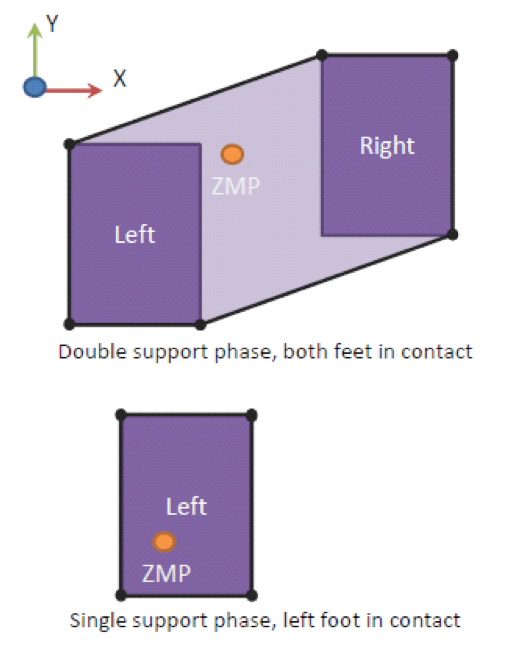
\includegraphics[width=0.5\columnwidth]{./background/pix/zmp.png}
  \caption{Example of the zero moment point on a bipedal robot in a single support phase (bottom) and a double support phase (top).  
If the zero moment point, the location of the center of mass (COM) projected in the direction of gravity, is located within this support polygon then the system is considered statically stable.}
  \label{fig:zmp}
\end{figure}

\noindent \textbf{Single Support Phase}:
The single support phase of a bipedal robot is when a single foot is touching the ground.
This creates a smaller support polygon.

\noindent \textbf{Double Support Phase}:
The double support phase of a bipedal robot is when two feed of a bipedal robot are on the ground.
This creates a larger support polygon.  
In addition there is a stable path that the ZMP can move from above one foot to the other.
This allows the robot to guarantee stability while walking (static walking).


		%% add other system comparisions?
